% Section owned by B (Dylan): theory, convergence, regularization, our checks.
\section{Theory: convergence and regularization}\label{sec:theory}

The iteration of Section~2,
$F(t+1) = \alpha S F(t) + (1-\alpha) Y$ with $S = D^{-1/2} W D^{-1/2}$,
converges because of what the symmetric normalization buys: $S$ is similar to the
row-stochastic matrix $D^{-1}W$, so its eigenvalues share those of a stochastic
matrix, and being symmetric they are real, all in $[-1,1]$ with top eigenvalue
exactly $1$. Hence for $\alpha \in (0,1)$ the spectral radius of $\alpha S$ is
$\alpha < 1$, the Neumann series $\sum_{i\ge 0}(\alpha S)^i = (I - \alpha S)^{-1}$
converges, and iterating from any starting point gives
\begin{equation}
  F^{*} = (1-\alpha)\,(I - \alpha S)^{-1}\, Y ,
  \label{eq:fixedpoint}
\end{equation}
the paper's closed form (its Eq.~3 up to the constant $1-\alpha$, which does not
affect the argmax rule). Writing $F(t) - F^{*} = (\alpha S)^{t}\,(F(0) - F^{*})$
shows both advertised properties at once: the limit is independent of $F(0)$, and
the error decays geometrically at rate $\alpha$.

Equation~\eqref{eq:fixedpoint} is not a lucky coincidence of the iteration; it is
the unique global minimiser of a regularised objective. With
$\mathcal{Q}(F) = \tfrac12 \sum_{i,j} W_{ij}
\bigl\|\tfrac{F_i}{\sqrt{D_{ii}}} - \tfrac{F_j}{\sqrt{D_{jj}}}\bigr\|^{2}
+ \mu \sum_i \|F_i - Y_i\|^{2}$ (the paper's Eq.~4), setting $\partial\mathcal{Q}/\partial F = 0$
gives $F - SF + \mu(F - Y) = 0$, and the substitution $\alpha = 1/(1+ \mu)$,
$\beta = \mu/(1+\mu) = 1-\alpha$ turns it into
$(I - \alpha S) F^{*} = \beta Y$: exactly the iteration's fixed point. The first
term is the graph-Laplacian smoothness energy in the degree-normalised coordinates
(it equals $\operatorname{tr}(F^{\top}(I-S)F)$), the second keeps predictions near
the clamped labels, and $\mu$ is the familiar regularisation trade-off strength:
ridge-regression structure with the Laplacian in place of the weight penalty.
The same normalisation appears one step earlier in spectral clustering
\citep{ng2001spectral}, and the manifold-regularisation framework of
\citet{belkin2004manifold} is the general form this paper instantiates on a graph;
compared to the harmonic-function method of \citet{zhu2003harmonic}, this algorithm
keeps the clamping term instead of imposing harmonicity.

\paragraph{Verification.}
We checked these claims numerically rather than trusting the derivation
(\texttt{experiments/convergence\_check.py}, results in
\texttt{results/\allowbreak convergence\_check\_summary.md}). Iterating to the residual tolerance
$10^{-12}$ agrees with solving the linear system directly to
$8\times10^{-11}$ max-abs on Role C's ten fixed two-moons trials, with zero argmax
disagreements; the observed stopping error equals $\mathrm{tol}/(1-\alpha)$ in every
run, because the residual criterion $\|F(t+1)-F(t)\|$ carries an extra factor
$(1-\alpha)$ relative to the error $\|F(t)-F^{*}\|$. Stationarity of
$\mathcal{Q}$ at $F^{*}$ holds to $2\times10^{-17}$, and every random perturbation
of $F^{*}$ tested raised $\mathcal{Q}$. The measured error-decay slope sits slightly
steeper than the predicted $\ln\alpha$ ($-0.0132$ vs $-0.0101$ at $\alpha=0.99$):
the $\alpha^{t}$ worst case rides on the degree-weighted top eigenvector $D^{1/2}\mathbf{1}$,
whose component of $F(0)-F^{*}$ nearly cancels here, so the next eigenvalue
dominates in practice (Figure~\ref{fig:rate}).

\begin{figure}[t]
  \centering
  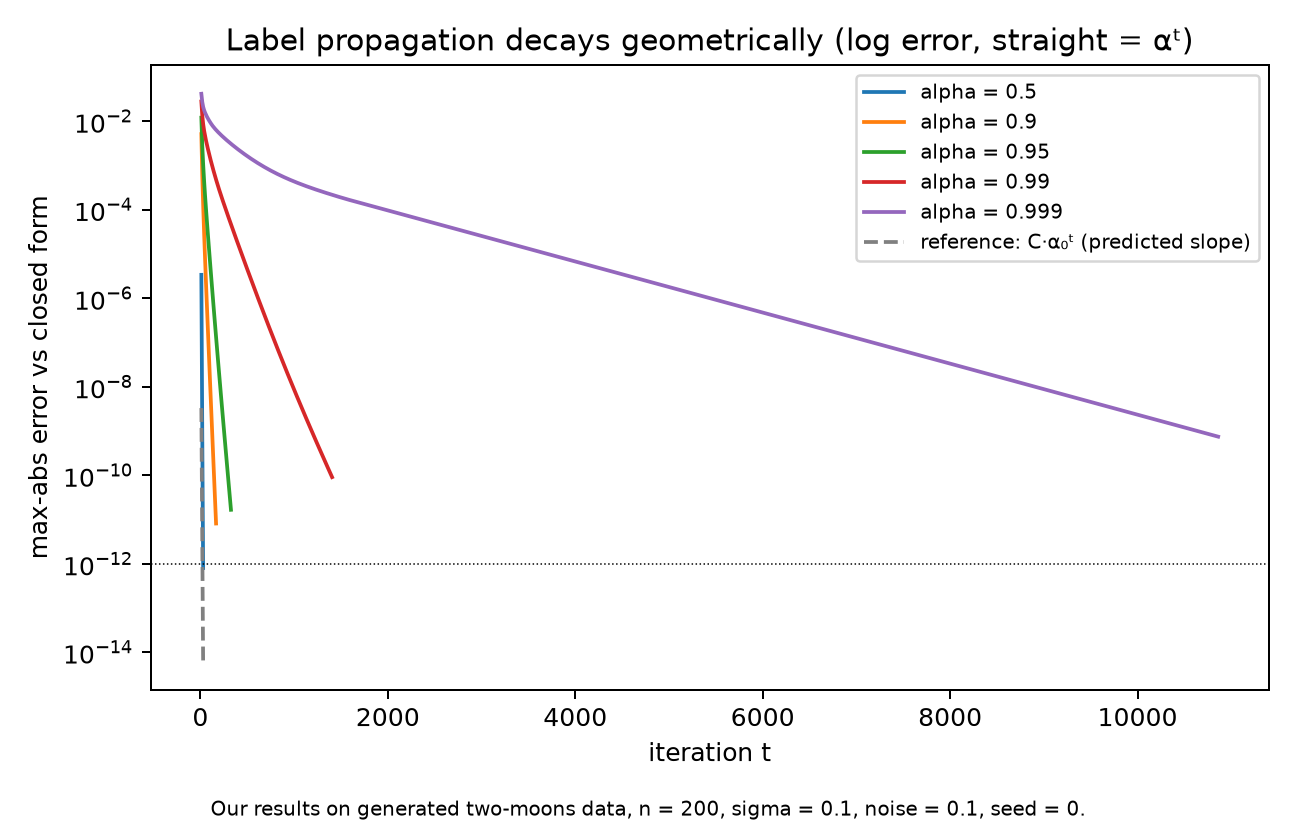
\includegraphics[width=0.72\linewidth]{../results/convergence_rate.png}
  \caption{Log max-abs error of the iteration against the closed form, for four
  values of $\alpha$, on our generated two-moons data. Straight lines confirm the
  geometric decay; the dashed line is the predicted $\alpha_0^{t}$ rate. Our
  result, not the paper's.}
  \label{fig:rate}
\end{figure}

\paragraph{An equation check.}
The last paragraph of Section~2 of the paper claims the transpose variant is
``equivalent'' to $F^{*} = (D - \alpha W)^{-1} D Y$. As written it is not, as
matrices: measured relative gap $0.82$ on our graph. The identity that does hold
(verified to $3\times10^{-15}$) is $(I - \alpha P^{\top})^{-1} Y =
D\,(D - \alpha W)^{-1} Y$ with $P = D^{-1}W$; pre-multiplying by $D$ is a positive
per-row rescaling, so \emph{classifications} agree everywhere and the paper's
word ``equivalent'' is defensible for the argmax rule while the displayed formula
misplaces the $D$ factor. All operator variants ($S$-based, $P$-based,
$P^{\top}$-based, and $(D-\alpha W)^{-1}$ with or without $DY$) differ by at most
$6/200$ predicted points on our toy, a useful robustness observation: the
method's classification is far less sensitive to the normalisation choice than
the raw score matrices are. Full audit in \texttt{results/variants\_audit.csv}.
